\documentclass[
    iict, % Saisir le nom de l'institut rattaché
    iscl, % Saisir le nom de l'orientation
    % confidential, % Décommentez si le travail est confidentiel
]{heig-tb}

\usepackage[nooldvoltagedirection,european,americaninductors]{circuitikz}

\signature{signature.svg} % Remplacer par votre propre signature vectorielle.

\makenomenclature
\makenoidxglossaries
\makeindex

\addbibresource{bibliography.bib}

\usepackage{etoolbox}
\renewcommand\nomgroup[1]{%
  \item[\bfseries
  \ifstrequal{#1}{A}{Constantes physiques}{%
  \ifstrequal{#1}{B}{Groupes}{%
  \ifstrequal{#1}{C}{Autres Symboles}{}}}%
]}

\newcommand{\nomunit}[1]{%
\renewcommand{\nomentryend}{\hspace*{\fill}#1}}

\nomenclature[A, 02]{\(c\)}{\href{https://physics.nist.gov/cgi-bin/cuu/Value?c}
{Vitesse de la lumière dans le vide}
\nomunit{\SI{299792458}{\meter\per\second}}}

\nomenclature[A, 03]{\(h\)}{\href{https://physics.nist.gov/cgi-bin/cuu/Value?h}
{Constante de Planck}
\nomunit{\SI[group-digits=false]{6.62607015e-34}{\joule\per\hertz}}}

\nomenclature[A, 01]{\(G\)}{\href{https://physics.nist.gov/cgi-bin/cuu/Value?bg}
{Constante de gravitation universelle}
\nomunit{\SI[group-digits=false]{6.67430e-11}{\meter\cubed\per\kilogram\per\second\squared}}}

\nomenclature[B, 03]{\(\mathbb{R}\)}{Nombres réels}
\nomenclature[B, 02]{\(\mathbb{C}\)}{Nombres complexes}
\nomenclature[B, 01]{\(\mathbb{H}\)}{Quaternions}

\nomenclature[C]{\(V\)}{Volume constant}
\nomenclature[C]{\(\rho\)}{Indice de frottement sec}

\newacronym{gcd}{GCD}{Plus grand diviseur commun}
\newacronym{lcm}{LCM}{Plus petit multiple commun}

\newglossaryentry{MitM}{
    name=MitM,
    description={Man in the Middle, attaque qui consiste à se placer entre deux interlocuteurs afin de récupérer des informations}
}

\newglossaryentry{ECDH}{
    name=ECDH,
    description={Elliptic Curve Diffie-Hellman, algorithme de génération de clés utilisant des courbes elliptiques}
}

\newglossaryentry{ECDSA}{
    name=ECDSA,
    description={Elliptic Curve Digital Signature Algorithm, algorithme de signature numérique utilisant des courbes elliptiques}
}

\newglossaryentry{PBKDF2}{
    name=PBKDF2,
    description={Password-Based Key Derivation Function 2, algorithme de dérivation de clés à partir d'un mot de passe}
}

\newglossaryentry{AES}{
    name=AES,
    description={Advanced Encryption Standard, algorithme de chiffrement par blocs}
}

\newglossaryentry{PWA}{
    name=PWA,
    description={Progressive Web Application, application web qui peut être installée sur un appareil et utilisée hors ligne}
}

\newglossaryentry{W3C}{
    name=W3C,
    description={World Wide Web Consortium, organisation à but non lucratif qui développe des standards pour le web}
}

\newglossaryentry{CRDT}{
    name=CRDT,
    description={Conflict-free Replicated Data Type, structure de données répliquée qui peut être mise à jour de manière indépendante et converger vers un état cohérent}
}

\newglossaryentry{DOM}{
    name=DOM,
    description={Document Object Model, interface de programmation pour les documents HTML et XML}
}

\newglossaryentry{TCP}{
    name=TCP,
    description={Transmission Control Protocol, protocole de transport fiable}
}

\newglossaryentry{WebRTC}{
    name=WebRTC,
    description={Web Real-Time Communication, API pour la communication en temps réel entre navigateurs}
}

\newglossaryentry{WebSocket}{
    name=WebSocket,
    description={Protocole de communication bidirectionnel, full-duplex, sur un seul socket TCP}
}

\newglossaryentry{DDnet}{
    name=DDnet,
    description={Decentralized Document Network, système réalisé dans le cadre de ce projet}
}

\newglossaryentry{Describble}{
    name=Describble,
    description={Nom de l'application réalisée dans le cadre de ce projet}
}

\newglossaryentry{DNS}{
    name=DNS,
    description={Domain Name System, système de noms de domaine, permet de faire la correspondance entre un nom de domaine et une adresse IP}
}
% Auteur du document (étudiant-e) en projet de Bachelor
\author{Maxime Scharwath}

% Activer l'option pour l'accord du féminin dans le texte
\genre{male}

% Titre de votre travail de Bachelor
\title{Edition collaborative de documents structurés avec un chiffrement de bout-en-bout et un stockage distribué}

% Le sous titre est optionnel
\subtitle{Travail de Bachelor}

% Nom du professeur responsable
\teacher {Prof. Chapuis Bertil (HEIG-VD)}

% Mettre à jour avec la date de rendu du travail
\date{\today}

% Numéro de TB
\thesis{7212}



\surroundwithmdframed{minted}

%% Début du document
\begin{document}
\selectlanguage{french}
\maketitle
\frontmatter
\clearemptydoublepage

%% Requis par les dispositions générales des travaux de Bachelor
\preamble
\authentification

%% Résumé / Résumé publiable / Version abrégée
\begin{abstract}
  % Francais
\lipsum[1]

\asterism

% English
\lipsum[3]

\end{abstract}

\begin{requirements}
  \section*{Présentation}
L'objectif principal de ce travail est de contribuer au développement de la startup Condensation en construisant un démonstrateur qui permettra de mettre en lumière les fonctionnalités du système, et de fournir aux développeurs des exemples concrets pour les aider à implémenter efficacement la librairie Condensation.

Pour atteindre cet objectif, plusieurs exemples seront développés pour exploiter les capacités du système de Condensation. Ces exemples seront regroupés sur une plateforme web complète et intuitive, accompagnée d'une documentation claire et précise qui fournira des explications détaillées sur l'utilisation de chaque exemple, ainsi que des tutoriels pour aider les développeurs à intégrer la librairie Condensation dans leurs projets.

Le résultat final de ce travail sera donc une solution clé en main pour les développeurs qui souhaitent utiliser le système de Condensation. Le démonstrateur développé constituera un outil précieux pour faciliter l'adoption du système, et contribuera ainsi au développement de la librairie en tant que solution de référence pour la synchronisation de données distribuées.

\section*{Livrables}
Les livrables à réaliser pour ce travail de bachelor sont les suivants:

\begin{itemize}
    \item Un rapport intermédiaire,
    \item Un rapport final,
    \item Un résumé publiable,
    \item Un poster,
    \item Un démonstrateur fonctionnel basé sur la librairie de Condensation permettant de mettre en évidence les fonctionnalités du système.
    \item Une plateforme web permettant de regrouper l'ensemble des modules développés, avec une documentation et tutoriels détaillés.
\end{itemize}

\section*{Objectifs}
Ce projet va répondre à plusieurs objectifs, répartis en 3 catégories : les objectifs \textbf{fonctionnels}, qui décrivent les fonctionnalités attendues du système, les objectifs \textbf{non-fonctionnels}, qui décrivent les caractéristiques de performance, de sécurité et d'accessibilité du système, et les objectifs \textbf{complémentaires, ou "nice-to-have"}, qui décrivent les fonctionnalités souhaitables mais non essentielles du système.

\subsection*{Objectifs \guillemotleft fonctionnels\guillemotright}

\begin{itemize}
    \item Développer plusieurs modules utilisant le système de Condensation qui permettront d'illustrer les fonctionnalités du système et de montrer aux développeurs comment les implémenter de manière efficace.
    \item Un exemple conséquent permettant l’édition d’un Whiteboard simultanément avec d’autres navigateurs, avec gestion des déconnexions inattendues, support de l’édition en mode “hors-ligne”, et doit pouvoir être partagé facilement.
    \item Regrouper les exemples sur une plateforme web complète et intuitive, offrant une expérience utilisateur optimale.
    \item Fournir une documentation claire et précise sera fournie pour chaque module, comprenant des tutoriels pour aider les développeurs à comprendre comment les intégrer dans leurs projets.
    \item Fournir deux serveurs de stoquage de données, pour permettre aux utilisateurs de choisir où stocker leurs données.
\end{itemize}


\subsection*{Objectifs \guillemotleft non-fonctionnels\guillemotright}

\begin{itemize}
    \item Concevoir une interface utilisateur intuitive, afin de permettre aux développeurs de tout de suite comprendre le fonctionnement des exemples.
    \item Garantir que le système peut être facilement étendu et adapté aux besoins futurs en utilisant des architectures évolutives et modulaires.
    \item S'assurer que le système est accessible aux utilisateurs de toutes les capacités, notamment en respectant les normes d'accessibilité et en prenant en compte les différents types d'appareils et de plateformes.
    \item 
\end{itemize}

\subsection*{Objectifs \guillemotleft complémentaires\guillemotright}

\begin{itemize}
    \item Ajouter d’autres exemples plus complexes.
    \item Offrir une interface multilingue pour la plateforme, afin de la rendre accessible à un public plus large.
\end{itemize}

\section*{Contraintes}
Cependant, il est important de noter que la librairie de Condensation est encore en développement. Pour éviter de perdre du temps sur le développement, un système de mock\footnote{Un mock de l'anglais \textit{mock-up}, qui signifie \textit{maquette}. Un mock est un objet qui simule le comportement d'un autre objet dans un contexte donné.} sera introduit pour simuler les interactions avec la librairie, tout en conservant la possibilité de l'intégrer facilement une fois qu'elle sera prête. Cette contrainte sera prise en compte dans la planification et l'exécution du projet.
\end{requirements}

%% Sommaire et tables
\clearemptydoublepage
{
  \tableofcontents
  %\let\cleardoublepage\clearpage
  %\listoffigures
  %\let\cleardoublepage\clearpage
  %\listoftables
  %\let\cleardoublepage\clearpage
  %\listoflistings
}

\printnomenclature
\clearemptydoublepage
\pagenumbering{arabic}

%% Contenu
\mainmatter
\chapter{Introduction}
\section{Contexte et introduction}

Le développement de solutions pour la synchronisation et la réplication de données distribuées est un défi majeur dans le domaine de l'informatique moderne. S'attaquant à ce défi, Condensation, une startup innovante, a créé une gamme de logiciels dédiés à garantir la cohérence des données à travers un réseau de n\oe{}uds. Leur système de synchronisation sans conflit assure l'intégrité des données et une sécurité de bout en bout.

L'architecture initiale de Condensation a été conçue par \textbf{Thomas Lochmatter} et est actuellement maintenue et développée par la startup elle-même. L'enjeu de la synchronisation des données distribuées rend ce projet particulièrement stimulant, notamment en raison des limites des solutions existantes.

Initialement, ce travail de Bachelor visait à collaborer avec Condensation pour développer un démonstrateur utilisant leur système. Cet outil aurait été conçu pour mettre en valeur les fonctionnalités du système et fournir aux développeurs des exemples concrets pour faciliter l'intégration de la bibliothèque dans leurs projets. Cependant, en raison d'une restructuration interne à Condensation, notamment leur décision de réécrire leur système en Rust, cette collaboration n'a pas pu se concrétiser comme prévu.

Face à cette situation, la direction de ce projet de Bachelor a dû être révisée. Au lieu d'utiliser le système existant de Condensation, il a fallu développer de A à Z un système de synchronisation et de réplication de données distribuées. Ce changement d'orientation a entraîné une augmentation significative du travail nécessaire pour ce projet. Cependant, cela a aussi créé une opportunité unique d'apprentissage et de développement de compétences techniques avancées.

En plus du développement de ce nouveau système, une application de création de whiteboard a été conçue pour illustrer son utilisation pratique. Le défi de créer à la fois le système et une application utilisant ce système a été une expérience très stimulante. Je suis particulièrement fier de ces réalisations et je suis enthousiaste à l'idée de les présenter dans ce rapport.

Bien que la collaboration directe avec Condensation n'ait pas eu lieu comme prévu, les principes et l'approche de Condensation ont eu une influence significative sur ce travail. Ce rapport décrira donc les différentes étapes de ce projet réorienté, les choix techniques réalisés, ainsi que les défis rencontrés et les solutions apportées.

\chapter{État de l'art}
\section{Définitions}
\subsection{Document structuré}
Un document structuré organise l'information de manière hiérarchique avec des éléments et attributs spécifiques. Il facilite la compréhension, la manipulation et la réutilisation des informations, contrairement aux documents non structurés.

Dans un tableau blanc collaboratif, un document structuré représente les éléments graphiques et textuels. Il aide à manipuler et modifier les éléments individuels, gérer l'historique des modifications et synchroniser les données entre les participants.

Le format SVG qui utilise le langage XML est un exemple de document structuré. Il est utilisé pour décrire la structure et le contenu d'un document vectoriel. Il est composé d'éléments graphiques, tels que des rectangles, des cercles et des lignes, et de textes.

\begin{listing}[H]
    \inputminted{XML}{assets/code/svg-example.svg}
    \caption{Exemple de document SVG \label{fig:svg-example}}
\end{listing}

\subsection{Édition collaborative de documents}
L'édition collaborative permet à plusieurs utilisateurs de travailler simultanément sur un document en fusionnant les modifications en temps réel.
Plusieurs outils existent pour l'édition collaborative de documents structurés, un exemple connu est Google Docs.

\section{Méthodes et protocoles pour resoudre les conflits de modification}
Lors de l'édition collaborative de documents structurés, les utilisateurs
peuvent modifier le document en même temps. Les modifications peuvent être
effectuées sur des éléments différents ou sur le même élément. Dans ce cas, il y
a un conflit de modification. Les conflits de modification peuvent être résolus
de différentes manières, par exemple en utilisant un mécanisme de verrouillage
ou en utilisant un algorithme de fusion. Dans les sections suivantes, nous
allons aborder les concepts clés, les mécanismes et les systèmes basés sur ces méthodes.

\subsection{Operational Transformation (OT)}
La Transformation Opérationnelle (OT) est un mécanisme de synchronisation de données en temps réel qui résout les conflits entre modifications concurrentes apportées par les utilisateurs. L'OT repose sur la transformation des opérations pour préserver leur intention lorsqu'elles sont appliquées dans un ordre différent. Dans cette section, nous aborderons les concepts clés, les mécanismes et les systèmes basés sur l'OT.

\subsubsection{Concepts de base de l'OT}
Pour comprendre le fonctionnement de l'OT, il est important de se familiariser avec les concepts de base suivants:

\paragraph{Opération:} Une opération est une action effectuée par un utilisateur sur un document, telle que l'insertion ou la suppression d'un caractère. Les opérations sont généralement représentées par des objets contenant des informations sur l'action effectuée, la position dans le document et, le cas échéant, le caractère inséré ou supprimé.
\paragraph{Intention:} L'intention d'une opération est l'effet souhaité de l'opération sur le document. L'OT vise à préserver l'intention des opérations, même lorsqu'elles sont appliquées dans un ordre différent.
\paragraph{Conflit:} Un conflit se produit lorsque deux opérations sont effectuées simultanément sur le même document, et que l'application de ces opérations dans un ordre différent peut entraîner des résultats incohérents. L'OT résout les conflits en transformant les opérations concurrentes de manière à préserver leur intention.

\subsubsection{Transformation des opérations et Conditions de transformation}
La transformation des opérations (OT) permet de préserver l'intention des opérations concurrentes en les modifiant. Supposons que deux utilisateurs, Alice et Bob, travaillent sur un document. Les opérations d'Alice et de Bob sont notées $O_A$ et $O_B$ respectivement. L'OT utilise les fonctions de transformation $T_1$ et $T_2$ pour résoudre les conflits, tel que :

\begin{equation}
    \begin{aligned}
        O_A' = T_1(O_A, O_B) \\
        O_B' = T_2(O_B, O_A)
    \end{aligned}
\end{equation}

Où $O_A'$ et $O_B'$ sont les opérations transformées. L'application de $O_A'$ et $O_B'$ sur le document préserve l'intention et résout les conflits.

Pour garantir que les opérations transformées sont cohérentes, peu importe l'ordre d'application, l'algorithme OT définit des propriétés de transformation (TP). Ces conditions, parfois appelées commutativité et idempotence, peuvent s'écrire :

\begin{equation}
    \begin{aligned}
        T_1(O_A', O_B') = O_A \\
        T_2(O_B', O_A') = O_B
    \end{aligned}
\end{equation}

Cela signifie que les opérations initiales $O_A$ et $O_B$ sont retrouvées en transformant à nouveau les opérations transformées $O_A'$ et $O_B'$ l'une par rapport à l'autre.

En définissant ces conditions de transformation appropriées, l'algorithme OT préserve les intentions des utilisateurs et garantit un document final cohérent, même en cas de travail simultané sur un même document.

\subsubsection{Algorithmes basés sur l'OT}
Plusieurs algorithmes et systèmes basés sur l'OT ont été développés, notamment Jupiter et Google Wave.

Jupiter est un système de collaboration en temps réel OT, créé au début des années 1990 au Xerox PARC. Il fonctionne en client-serveur, chaque client et serveur possédant sa propre copie du document et appliquant les opérations localement.

Google Wave était un système de collaboration en temps réel conçu par Google, basé sur l'OT. Il utilisait un modèle décentralisé où chaque utilisateur maintenait sa propre copie du document, offrant plus de flexibilité pour gérer les modifications hors ligne et synchroniser les données lorsqu'un utilisateur se reconnectait.

Cependant, Google Wave ne parvint pas à attirer suffisamment d'utilisateurs et son développement fut arrêté. Néanmoins, certaines idées et techniques furent intégrées dans d'autres produits de collaboration en temps réel de Google, tels que Google Docs.

\subsubsection{Limitations et défis de l'OT}
Bien que l'OT soit un mécanisme puissant pour la synchronisation en temps réel des documents et la résolution des conflits, il présente également certaines limitations et défis. Par exemple, les algorithmes basés sur l'OT peuvent être complexes à mettre en oeuvre et à déboguer, particulièrement lorsqu'ils doivent gérer des cas de conflits complexes et des relations de causalité. De plus, la transformation des opérations et le contrôle de la causalité peuvent avoir un impact sur les performances, surtout lorsque le nombre d'utilisateurs et d'opérations concurrentes augmente. Malgré ces défis, l'OT reste une méthode importante et largement utilisée pour la collaboration en temps réel et la synchronisation des données dans les systèmes distribués.

\subsection{Conflict-Free Replicated Data Types (CRDT)}
Les Conflict-Free Replicated Data Types sont des structures de données distribuées qui facilitent la collaboration en temps réel sur des données partagées sans nécessiter un serveur central. Les opérations sur les \Gls{CRDT} sont commutatives et idempotentes, assurant ainsi une convergence stable et une cohérence des données dans un environnement distribué.

\subsubsection{Principes des \Gls{CRDT}}
Les \Gls{CRDT} sont distribués et répliqués sur plusieurs noeuds, chaque noeud possédant une copie des données. Les noeuds peuvent modifier les données localement et les synchroniser entre eux. Chaque opération est associée à un identifiant unique pour garantir la commutativité et l'idempotence des opérations.

\subsubsection{Exemple d'application des \Gls{CRDT} : Logoot}
Pour illustrer le fonctionnement des \Gls{CRDT}, considérons le cas de Logoot, un type de \Gls{CRDT} conçu pour la collaboration en temps réel sur des documents textuels. Dans l'algorithme Logoot, chaque caractère dans le document est associé à un identifiant unique, qui est une paire d'éléments notée sous la forme `(x, y)`. Le premier élément `x` correspond à la position du caractère dans le document, tandis que le second élément `y` est un identifiant unique généré lors de l'insertion du caractère.

Prenons l'exemple de deux utilisateurs, Alice et Bob, collaborant sur un document texte initialisé avec le mot "chat".

\paragraph{Scénario}
Alice et Bob travaillent sur un texte initial "chat". Alice veut former "chou" en ajoutant "ou" après "ch", pendant que Bob veut former "chef" en ajoutant "ef" après "ch".

\paragraph{Logoot \Gls{CRDT}}
Nous illustrons ci-dessous comment Alice et Bob peuvent collaborer sur le document texte en utilisant Logoot \Gls{CRDT} :

Le document initial est :

\begin{equation}
    c(1),\ h(2), \ a(3), t(4) \quad \text{(chat)}
\end{equation}

Ici, chaque caractère du document est suivi d'une paire d'éléments `(x, y)`, où `x` est la position du caractère dans le document et `y` est un identifiant unique généré lors de l'insertion du caractère.

\paragraph{Opérations d'insertion}
Alice insère "ou" après "ch" et génère de nouvelles positions :

\begin{equation}
    o(2, 1), \ u(2, 2)
\end{equation}

Le texte d'Alice devient :

\begin{equation}
    c(1), \ h(2), \ o(2, 1), \ u(2, 2), \ a(3), \ t(4) \quad \text{(chouat)}
\end{equation}

Bob insère "ef" après "ch" et génère aussi de nouvelles positions :

\begin{equation}
    e(2, 3), f(2, 4)
\end{equation}

Le texte de Bob devient :

\begin{equation}
    c(1), \ h(2), \ e(2, 3), \ f(2, 4), \ a(3), \ t(4) \quad \text{(chefat)}
\end{equation}

\paragraph{Intégration des opérations}
Les opérations d'insertion sont ensuite échangées. Alice intègre l'insertion de Bob, et Bob intègre l'insertion d'Alice. Le résultat est identique pour Alice et Bob, malgré un ordre différent d'opérations. Les CRDT assurent convergence et cohérence sans transformation opérationnelle.

\subsubsection{Applications des \Gls{CRDT}}
Les \Gls{CRDT} inspirent de nombreux algorithmes et systèmes de collaboration en temps réel, tels que WOOT, Treedoc, RGA, Logoot, LSEQ, Automerge et Yjs.

\paragraph{Automerge\cite{hardenbergAutomerge2023}: } Automerge est une bibliothèque JavaScript pour développer des applications collaboratives en temps réel, comme des éditeurs de texte et des tableaux Kanban. Elle utilise des \Gls{CRDT} pour synchroniser les données entre les instances de l'application, en maintenant la cohérence et en résolvant les conflits.

\paragraph{Yjs\cite{nicolaescuYjsFrameworkRealTime2015}: } Yjs est une bibliothèque JavaScript de collaboration en temps réel qui utilise aussi les \Gls{CRDT} pour la synchronisation des données. Yjs supporte diverses structures de données et fonctionnalités, dont la collaboration sur des documents texte, des tableaux et des graphes.

En résumé, les \Gls{CRDT} sont une approche puissante pour la collaboration en temps réel. Elles résolvent les problèmes de synchronisation et de cohérence des données sans recourir à la transformation opérationnelle. Cependant, elles ne sont pas adaptées à tous les types de données et structures de données, et leur mise en oeuvre peut être complexe.

\section{Zéro Trust}
Le modèle Zéro Trust est une approche de cybersécurité basée sur l'idée de ne faire confiance à aucune entité, interne ou externe, dans un système informatique. On vérifie constamment les identités et les autorisations avant d'accorder l'accès aux ressources. Cette méthode réduit les risques de failles de sécurité et protège les données sensibles contre les accès non autorisés.

\section{Chiffrement de bout en bout}

Avec l'ère numérique, il est devenu primordial de sécuriser nos communications pour les protéger des intermédiaires tels que les fournisseurs de services Internet (FSI) et les fournisseurs de services tels que Whatsapp, Telegram ou Signal, qui sont tous en position d'intercepter, d'enregistrer et même de modifier nos communications sans notre consentement ou notre connaissance.

Dans ce contexte, le chiffrement de bout en bout (E2EE) est essentiel. L'E2EE garantit que seuls les destinataires prévus sont capables de déchiffrer et de lire les messages. Ainsi, aucun des intermédiaires ne peut inspecter, stocker ou modifier vos messages privés.

\subsection{Cryptographie à clé publique et cryptographie symétrique}

Il est important de comprendre que le terme \textit{"message"} ne se réfère pas uniquement à un courrier électronique ou à un message de chat. Il peut également s'agir d'un paquet réseau, c'est-à-dire de tout ce que vous faites en ligne, de la visite de sites web à l'achat de chaussures en passant par les jeux en ligne.

Le message d'origine est appelé texte en clair, et le message chiffré est appelé texte chiffré. Pour chiffrer un message de manière à ce que seul notre cher ami Bob puisse le déchiffrer, nous avons besoin d'utiliser la cryptographie à clé publique, également appelée cryptographie asymétrique.

La cryptographie à clé publique est basée sur le principe des clés de chiffrement en paires :

\begin{itemize}
    \item Une clé publique est une clé qui doit être partagée avec d'autres afin qu'ils puissent l'utiliser pour chiffrer des données destinées à vous, et à vous seul.
    \item Une clé privée est un secret qui ne doit jamais être partagé avec personne et qui vous permet de déchiffrer les données qui ont été préalablement chiffrées avec la clé publique.
\end{itemize}

La réalité est que le chiffrement à clé publique est limité par la longueur des messages qu'il peut chiffrer et qu'il est douloureusement lent. C'est là qu'intervient le chiffrement hybride. Le chiffrement hybride prend le meilleur du chiffrement symétrique et du chiffrement asymétrique : les messages sont chiffrés avec le chiffrement symétrique (rapide, de toute longueur, sûr...), et seule la clé secrète symétrique éphémère (courte, de 256 bits - 32 octets la plupart du temps) est chiffrée à l'aide du chiffrement asymétrique.

\subsection{Échange de clés Diffie–Hellman et Sécurité Avancée}

Pour garantir une sécurité optimale, la clé doit être renouvelée pour chaque nouveau message. De plus, il est recommandé d'utiliser le chiffrement authentifié avec des données associées (AEAD, pour Authenticated Encryption with Associated Data) qui nous permet de détecter si le texte chiffré a été modifié.

Malgré ces mesures, la situation n'est toujours pas parfaite. Les clés RSA ont tendance à être grandes (3072 bits ou plus), et le chiffrement RSA n'est pas facile à bien faire, ce qui est une grande source d'erreurs.

Pour remédier à cela, on utilise l'échange de clés Diffie–Hellman (plus couramment appelé échange de clés). Il s'agit d'une méthode pour établir un secret partagé entre deux parties par le biais d'un canal public. L'échange de clés Diffie–Hellman est beaucoup plus simple à mettre en oeuvre que le chiffrement RSA.

Toutefois, les secrets partagés calculés par l'échange de clés Diffie–Hellman ne peuvent pas être utilisés directement pour le chiffrement symétrique. La plupart des algorithmes AEAD attendent une clé symétrique aléatoire uniforme, ce que ne sont pas les secrets partagés. Ainsi, pour "augmenter leur entropie", nous passons la sortie de la fonction d'échange de clés dans une fonction de dérivation de clés (KDF, pour Key Derivation Function) pour générer une clé secrète partagée qui peut être utilisée pour le chiffrement symétrique.

Mais qu'arrive-t-il si notre clé privée est divulguée ? Si un intermédiaire a enregistré tous nos messages et que notre clé privée fuit, un acteur malveillant serait en mesure de déchiffrer tous les messages ! Passé, présent et futur.

Pour remédier à cela, nous utilisons la Sécurité Avancée (aussi connue sous le nom de Sécurité Avancée Parfaite). C'est une caractéristique des protocoles qui garantit que si une clé fuite à l'instant T, les messages envoyés avant, à T-1, T-2, T-3... ne peuvent pas être déchiffrés.

\subsection{Signatures numériques}

Pour mettre en oeuvre la Sécurité Avancée, on pourrait simplement créer de nombreuses paires de clés, utiliser une paire de clés par message et la supprimer une fois le message reçu. Mais alors, nous perdons notre fonctionnalité selon laquelle 1 clé publique = 1 identité : nous devrions vérifier avec Bob pour chaque message que chaque clé publique est légitime et provient réellement de Bob, et non d'un attaquant \Gls{MitM} (Man in the Middle), ce qui est impraticable.

Pour résoudre ce problème, nous utilisons des signatures. Les signatures permettent à une personne en possession d'une clé privée d'authentifier un document ou un message. En signant le message ou le document, le propriétaire de la clé privée atteste de sa validité. Ensuite, tout le monde qui a accès à la clé publique peut vérifier que la signature correspond au document.

Ainsi, les signatures sont l'outil parfait pour créer une identité numérique.

En résumé, le chiffrement moderne de bout en bout = Signatures + Échange de clés + AEAD

\section{Conclusion}
En conclusion, l'état de l'art dans le domaine de l'édition collaborative de
documents, du chiffrement de bout en bout et du stockage distribué montre qu'il
existe plusieurs approches pour aborder ces problématiques. Les systèmes basés
sur resolution de conflits, tels que Jupiter et Google Wave, ont apporté des
contributions significatives dans la synchronisation des données en temps réel
et la résolution des conflits. Cependant, des défis subsistent, tels que la
complexité et les performances des algorithmes.

Face à ces défis, les chercheurs et les développeurs continuent d'explorer de nouvelles approches et d'améliorer les technologies existantes pour répondre aux besoins croissants en matière de collaboration, de sécurité et de décentralisation des données.

\chapter{Aspect technique}
Dans ce chapitre, nous allons explorer en profondeur les aspects techniques de la mise en œuvre du projet, en examinant les technologies et les méthodes employées. Nous aborderons également l'intégration de la bibliothèque Condensation et la gestion du stockage des données.

\section{Monorepo}
Un monorepo, ou dépôt mono-référentiel, est une approche de gestion de code source qui consiste à stocker l'ensemble du code et des ressources d'un projet, y compris ses bibliothèques, ses composants et ses applications, dans un seul et même dépôt de contrôle de version. Cette approche contraste avec les polyrepos, où chaque projet, bibliothèque ou composant est stocké dans un dépôt séparé.

\subsection{Avantages}

L'utilisation d'un monorepo présente plusieurs avantages pour les grands projets, notamment :

\begin{itemize}
    \item \textbf{Gestion des dépendances simplifiée :} Dans un monorepo, toutes les versions des dépendances sont centralisées en un seul endroit, ce qui facilite leur gestion et leur mise à jour. Cela permet également de s'assurer que toutes les parties du projet utilisent des versions cohérentes des dépendances, évitant ainsi les problèmes de compatibilité.
    \item \textbf{Collaboration et communication améliorées :} Un monorepo encourage la collaboration entre les développeurs, car ils travaillent tous sur la même base de code. Cela facilite la découverte et la réutilisation des composants et des bibliothèques, et favorise une meilleure compréhension de l'ensemble du projet.
    \item \textbf{Intégration et tests simplifiés :} Dans un monorepo, il est plus facile d'assurer l'intégration et la cohérence des différentes parties du projet, car les modifications apportées à une partie du code peuvent être immédiatement testées et validées dans le contexte global du projet. Cela permet de détecter rapidement les régressions et les problèmes de compatibilité.
    \item \textbf{Historique et traçabilité unifiés :} Un monorepo conserve l'historique de l'ensemble du projet en un seul endroit, ce qui facilite la recherche et la compréhension des modifications apportées au fil du temps. Cela permet également de suivre les dépendances et les interactions entre les différentes parties du projet, ce qui peut être utile pour l'analyse d'impact et le débogage.
\end{itemize}

\subsection{Inconvénients}

Malgré ses avantages, l'utilisation d'un monorepo peut également présenter quelques inconvénients, tels que :

\begin{itemize}
    \item \textbf{Taille du dépôt :} Un monorepo peut devenir très volumineux, ce qui peut ralentir certaines opérations de contrôle de version et compliquer la gestion du dépôt.
    \item \textbf{Complexité de la configuration :} La configuration d'un monorepo peut être plus complexe que celle d'un polyrepo, notamment en ce qui concerne la gestion des dépendances, la configuration des outils de développement et l'automatisation des tests et des déploiements.
    \item \textbf{Séparation des responsabilités :} Dans un monorepo, il peut être plus difficile de maintenir une séparation claire des responsabilités entre les différentes parties du projet, et de contrôler l'accès et les autorisations des développeurs.
\end{itemize}

\section{TurboRepo}

TurboRepo est un système de construction hautes performances pour les projets TypeScript et JavaScript, conçu pour optimiser et accélérer les processus de construction dans les monorepos. Il offre plusieurs fonctionnalités puissantes, telles que :

\begin{itemize}
    \item Construction incrémentale rapide
    \item Mise en cache des calculs locaux
    \item Mise en cache des calculs distribués
    \item Orchestration des tâches locales
    \item Visualisation du graphe des dépendances
    \item Partage du code source
\end{itemize}

L'un des principaux avantages de TurboRepo est sa capacité à minimiser les temps d'inactivité du CPU et à accélérer les tâches grâce à une planification intelligente. Il est conçu pour être adopté de manière incrémentale, ce qui signifie qu'il peut être ajouté à un codebase existant en quelques minutes seulement.

\section{Gestionnaires de paquets et pnpm}

Un gestionnaire de paquets est un outil qui permet d'automatiser l'installation, la mise à niveau, la configuration et la désinstallation de paquets logiciels. Dans le contexte des projets Node.js, un gestionnaire de paquets gère les dépendances et les bibliothèques requises par le projet. Les gestionnaires de paquets aident à simplifier et à organiser le développement en fournissant un moyen structuré et centralisé de gérer les dépendances, ce qui améliore la maintenabilité et la reproductibilité des projets.

Les gestionnaires de paquets les plus couramment utilisés dans l'écosystème JavaScript et Node.js sont npm (Node Package Manager) et yarn. Ces outils permettent aux développeurs d'installer et de gérer les bibliothèques et les modules dont leurs projets ont besoin, en téléchargeant les paquets à partir d'un registre en ligne, généralement le registre npm.

\subsection{pnpm}

pnpm est un gestionnaire de paquets alternatif pour Node.js qui est compatible avec le registre npm. Il se distingue par son approche de stockage des paquets, qui utilise des liens durs et des liens symboliques pour créer un stockage partagé des paquets. Cela permet d'économiser de l'espace disque et de réduire les temps d'installation des paquets.

\subsection{Pourquoi choisir pnpm ?}

Il existe plusieurs raisons pour lesquelles vous pourriez choisir pnpm plutôt que d'autres gestionnaires de paquets comme npm ou yarn :

\begin{itemize}
    \item \textbf{Efficacité du stockage :} Comme mentionné précédemment, pnpm utilise des liens durs et des liens symboliques pour créer un stockage partagé des paquets. Cela signifie que chaque version d'un paquet n'est stockée qu'une seule fois sur le disque, même si elle est utilisée par plusieurs projets. Cela permet de réduire considérablement l'espace disque utilisé par les dépendances du projet.
    \item \textbf{Performances d'installation :} Grâce à son approche de stockage des paquets, pnpm peut réduire les temps d'installation en évitant de télécharger et d'extraire les mêmes paquets plusieurs fois. Les paquets sont simplement liés au projet, ce qui est beaucoup plus rapide que de les copier.
    \item \textbf{Garantie d'isolation :} pnpm garantit que les dépendances d'un projet sont strictement isolées des autres projets, ce qui évite les problèmes causés par les dépendances partagées ou les dépendances non déclarées. Cela permet de détecter et de corriger les erreurs de configuration des dépendances plus tôt dans le processus de développement.
    \item \textbf{Compatibilité :} pnpm est compatible avec le registre npm et les fichiers package.json standard, ce qui signifie qu'il peut être utilisé comme un remplacement direct pour npm ou yarn sans nécessiter de modifications importantes dans la configuration du projet.
\end{itemize}

En somme, pnpm est une alternative intéressante aux gestionnaires de paquets traditionnels comme npm ou yarn. Il offre des avantages en termes d'efficacité du stockage, de performances d'installation et d'isolation des dépendances, tout en restant compatible avec l'écosystème npm existant. L'utilisation de pnpm dans un grand projet peut entraîner des gains significatifs en matière d'espace disque et de temps d'installation, ainsi qu'une meilleure gestion et détection des problèmes liés aux dépendances.

\subsection{Intégration avec TurboRepo}

Comme mentionné précédemment, pnpm peut être utilisé en conjonction avec TurboRepo pour améliorer encore les performances et la gestion des dépendances dans un projet monorepo. TurboRepo se concentre sur l'exécution efficace des tâches de build et de test, tandis que pnpm gère l'installation et la gestion des paquets.

L'intégration de pnpm avec TurboRepo permet de tirer parti des avantages de chacun de ces outils pour créer une expérience de développement plus fluide et performante. TurboRepo peut utiliser les caches de build générés par pnpm pour éviter les tâches de build inutiles et accélérer les pipelines de build. En même temps, pnpm peut tirer parti de la structure monorepo et de la gestion des dépendances centralisée offerte par TurboRepo pour optimiser l'installation et la gestion des paquets.

En conclusion, l'utilisation de pnpm en combinaison avec TurboRepo dans un grand projet peut offrir une solution robuste et performante pour la gestion des dépendances et l'exécution des tâches de build. Les avantages de ces outils peuvent contribuer à améliorer la productivité et la maintenabilité du projet, tout en offrant une expérience de développement plus fluide et plus rapide.


\section{TypeScript}
TypeScript est un langage de programmation développé par Microsoft qui est un sur-ensemble typé de JavaScript. Cela signifie que tout code JavaScript est également du code TypeScript valide. TypeScript ajoute un système de typage statique optionnel à JavaScript, ce qui permet de détecter et d'éviter les erreurs de typage à la compilation plutôt qu'à l'exécution. Le code TypeScript est transcompilé en JavaScript, ce qui le rend compatible avec tous les navigateurs et environnements qui supportent JavaScript.

Dans cette section, nous expliquerons en profondeur ce qu'est TypeScript et pourquoi il est particulièrement utile et nécessaire dans les grands projets.

\subsection{Typage statique}
Le typage statique est l'un des principaux avantages de TypeScript par rapport à JavaScript. Contrairement à JavaScript, qui est un langage à typage dynamique, TypeScript permet de définir des types pour les variables, les fonctions, les objets et les classes. Cela permet au compilateur TypeScript de vérifier la conformité des types lors de la compilation et d'alerter le développeur en cas d'erreurs de typage.

Le typage statique présente plusieurs avantages pour les grands projets :

\begin{itemize}
    \item \textbf{Détection précoce des erreurs :} Le compilateur TypeScript peut détecter les erreurs de typage avant l'exécution du code, ce qui permet de les corriger plus rapidement et de réduire le nombre de bugs en production.
    \item \textbf{Documentation implicite :} Les types fournissent une documentation implicite pour le code, rendant plus facile la compréhension du code par les autres développeurs et facilitant la maintenance et l'évolution du projet.
    \item \textbf{Amélioration de l'autocomplétion et du refactoring :} Les outils de développement modernes peuvent utiliser les informations de type pour fournir une meilleure autocomplétion et faciliter le refactoring du code.
\end{itemize}

\subsection{Compatibilité avec JavaScript}

Comme TypeScript est un sur-ensemble de JavaScript, il est compatible avec tout le code JavaScript existant. Cela signifie que les développeurs peuvent migrer progressivement leur codebase vers TypeScript en ajoutant des types aux parties les plus critiques du code, sans avoir à réécrire l'ensemble de l'application.

Cette compatibilité permet également d'utiliser toutes les bibliothèques et frameworks JavaScript existants, tels que React, Angular et Vue.js, ainsi que les packages npm.

\subsection{Support des fonctionnalités modernes de JavaScript}

TypeScript supporte toutes les fonctionnalités modernes de JavaScript, telles que les classes, les modules, les décorateurs, les fonctions fléchées et les promesses. Il ajoute également des fonctionnalités supplémentaires, telles que les interfaces, les types génériques et les espaces de noms.

Cela permet aux développeurs d'utiliser les dernières fonctionnalités de JavaScript tout en bénéficiant des avantages du typage statique.

\subsection{Scalabilité et maintenabilité}

Dans les grands projets, la complexité du code et la taille de l'équipe de développement peuvent rendre difficile la maintenance et l'évolution du code. TypeScript facilite la gestion de cette complexité en fournissant un système de typage statique et des fonctionnalités avancées de modularisation.

Les avantages de TypeScript en termes de scalabilité et de maintenabilité incluent :

\begin{itemize}
    \item \textbf{Modularité :} TypeScript supporte les modules et les espaces de noms, ce qui permet de diviser le code en unités logiques et de faciliter la réutilisation des composants. Les modules TypeScript peuvent également être intégrés avec les systèmes de modules existants, tels que CommonJS et ES6.
    \item \textbf{Interfaces :} Les interfaces TypeScript permettent de définir des contrats entre les composants du code, garantissant que ces composants respectent les attentes en termes de types et de comportement. Les interfaces sont particulièrement utiles pour définir des API claires et cohérentes entre les différentes parties du code.
    \item \textbf{Types génériques :} Les types génériques permettent de créer des composants réutilisables qui peuvent fonctionner avec différents types de données, sans sacrifier la sécurité du typage. Les types génériques sont couramment utilisés pour définir des structures de données, des fonctions et des classes qui sont indépendantes du type de données qu'elles manipulent.
    \item \textbf{Refactoring :} Les outils de développement modernes peuvent tirer parti des informations de type fournies par TypeScript pour faciliter le refactoring du code. Cela permet de modifier la structure du code sans affecter son comportement, ce qui est essentiel pour la maintenabilité à long terme des grands projets.
\end{itemize}

\subsection{Communauté et écosystème}

TypeScript bénéficie d'une communauté active et en pleine croissance, qui contribue à son développement et à sa popularité. De nombreuses bibliothèques et frameworks JavaScript populaires, tels que React, Angular et Vue.js, supportent TypeScript nativement ou via des fichiers de déclaration de type, ce qui facilite son adoption.

De plus, la majorité des packages npm fournissent des fichiers de déclaration de type pour TypeScript, soit directement dans le package, soit via le dépôt DefinitelyTyped. Cela permet aux développeurs de bénéficier du typage statique lorsqu'ils utilisent des bibliothèques et des frameworks tiers.

\section{Frameworks frontend réactifs}

\subsection{Qu'est-ce qu'un framework frontend réactif ?}

Un framework frontend réactif est une bibliothèque ou un ensemble d'outils permettant de créer des applications Web modernes avec une interface utilisateur dynamique et réactive. Ces frameworks facilitent la manipulation du DOM (Document Object Model), la gestion des états, la communication avec les API backend et l'intégration d'autres fonctionnalités avancées. En outre, ils favorisent la modularité et la réutilisabilité du code en permettant aux développeurs de créer des composants réutilisables et indépendants.

\subsection{Pourquoi les frameworks frontend réactifs sont-ils utiles ?}

Les frameworks frontend réactifs offrent plusieurs avantages pour le développement d'applications Web, notamment :

\paragraph{Réactivité :} Ils permettent de créer des interfaces utilisateur dynamiques et réactives qui s'adaptent automatiquement aux modifications de l'état de l'application ou aux interactions de l'utilisateur.
\paragraph{Modularité et réutilisabilité :} Les frameworks réactifs encouragent la création de composants modulaires et réutilisables, ce qui facilite la maintenance et l'évolution du code, ainsi que la collaboration entre les développeurs.
\paragraph{Productivité :} Ils fournissent des outils et des abstractions pour simplifier le développement et réduire la quantité de code à écrire, ce qui améliore la productivité des développeurs.
\paragraph{Performances :} Les frameworks réactifs optimisent les performances en minimisant les mises à jour du DOM et en utilisant des techniques avancées, telles que la détection de changements, le rendu différé et la mise en cache intelligente.

\subsection{Pourquoi choisir React par rapport aux alternatives ?}

Plusieurs frameworks frontend réactifs sont disponibles, tels que React, Angular et Vue.js. Nous avons choisi React pour ce projet en raison de sa popularité, de sa large compatibilité avec les bibliothèques existantes et de son approche flexible et modulaire. Voici quelques raisons qui ont motivé notre choix :

\paragraph{Popularité :} React est l'un des frameworks frontend les plus populaires et largement utilisés, avec une grande communauté de développeurs et une vaste documentation. Cette popularité signifie que de nombreux problèmes et défis courants ont déjà été résolus par d'autres développeurs, et il existe de nombreuses ressources pour apprendre et se familiariser avec le framework.
\paragraph{Compatibilité avec les bibliothèques :} Grâce à sa popularité, React est compatible avec un grand nombre de bibliothèques et de plugins existants, ce qui facilite l'intégration de fonctionnalités supplémentaires dans notre projet sans avoir à réinventer la roue.
\paragraph{Approche flexible et modulaire :} React se concentre sur la création de composants réutilisables et indépendants, ce qui facilite la modularité et la réutilisabilité du code. Cette approche flexible permet de créer des applications à l'architecture claire et maintenable, tout en facilitant la collaboration entre les développeurs.
\paragraph{Performances :} React utilise un algorithme de réconciliation efficace et un DOM virtuel pour minimiser les mises à jour du DOM réel, ce qui améliore les performances de l'application. De plus, React prend en charge des fonctionnalités telles que le découpage de code et le chargement différé pour optimiser davantage les performances.

\paragraph{Ecosystème :} L'écosystème de React est riche et diversifié, offrant un grand nombre de bibliothèques, d'outils et de solutions pour résoudre divers problèmes de développement. Cela permet aux développeurs de se concentrer sur la logique métier de l'application plutôt que sur les détails techniques.

\paragraph{Mise à jour et maintenance :} React est développé et maintenu par Facebook, qui l'utilise dans ses propres applications. Cela signifie que React bénéficie d'un soutien solide, de mises à jour régulières et d'une maintenance à long terme.

\section{Utilisation de Tailwind CSS}

Tailwind CSS est un framework CSS moderne et très populaire qui se concentre sur l'utilité, la flexibilité et la personnalisation. Il est conçu pour faciliter la création de designs responsifs et cohérents en fournissant un ensemble de classes CSS préconfigurées qui peuvent être facilement combinées pour construire rapidement des interfaces utilisateur. Dans cette section, nous discuterons des avantages et des inconvénients de l'utilisation de Tailwind CSS, ainsi que des raisons pour lesquelles il a été choisi pour ce projet.

\subsection{Avantages}

\paragraph{Utilitaires basés sur des classes}

Tailwind CSS utilise une approche basée sur des classes utilitaires, ce qui permet de créer des styles directement dans le code HTML. Cela facilite la compréhension du style appliqué à un élément, car il n'est pas nécessaire de naviguer entre plusieurs fichiers CSS. Cette approche permet également une meilleure réutilisabilité et une maintenance plus facile des styles, car les classes utilitaires sont cohérentes et préconfigurées.

\paragraph{Personnalisation}

Tailwind CSS offre un haut degré de personnalisation grâce à son fichier de configuration. Les développeurs peuvent définir leurs propres valeurs pour les couleurs, les polices, les espacements et d'autres propriétés CSS. Cette personnalisation permet de créer des designs uniques et cohérents tout en bénéficiant de la facilité d'utilisation et de la rapidité de développement offerte par les classes utilitaires de Tailwind.

\paragraph{Optimisation des performances}

Tailwind CSS est livré avec des outils d'optimisation intégrés qui aident à réduire la taille du fichier CSS final. Par exemple, il utilise PurgeCSS pour supprimer automatiquement les classes CSS inutilisées du fichier de production. Cela garantit que seules les classes réellement utilisées dans le projet sont incluses dans le fichier CSS, réduisant ainsi la taille du fichier et améliorant les performances.

\subsection{Inconvénients}

\paragraph{Courbe d'apprentissage}

La documentation de Tailwind CSS est très complète et fournit de nombreuses ressources pour apprendre à utiliser le framework. S'il on est familiarisé avec Bootstrap, il est relativement facile de se familiariser avec Tailwind CSS. Cependant, il peut être difficile pour les développeurs qui n'ont jamais utilisé de framework CSS de comprendre comment fonctionne Tailwind CSS et comment l'utiliser pour créer des designs responsifs et cohérents. Il est donc judicieux de passer du temps à lire la documentation et à explorer les exemples fournis avant de commencer à utiliser Tailwind CSS dans un projet.

\paragraph{Verbosité}

L'utilisation de classes utilitaires peut rendre le code HTML plus verbeux, car chaque élément doit inclure toutes les classes nécessaires pour appliquer le style souhaité. Cela peut rendre le code HTML plus difficile à lire et à maintenir. Cependant, ce problème peut être atténué en extrayant les styles réutilisables dans des composants ou en utilisant des directives CSS personnalisées.

\subsection{Pourquoi choisir Tailwind CSS pour ce projet?}

Le choix de Tailwind CSS pour ce projet s'est avéré être une décision judicieuse, car il offre un grand nombre d'avantages et de fonctionnalités qui répondent aux besoins du projet. En plus de ses avantages évidents, tels que la facilité d'utilisation et la rapidité de développement, Tailwind CSS offre également une grande flexibilité et une personnalisation poussée, ce qui permet de créer des designs uniques et cohérents. De plus, Tailwind CSS est livré avec des outils d'optimisation intégrés qui aident à réduire la taille du fichier CSS final, ce qui améliore les performances de l'application.

\section{Gestion des états avec les stores React et l'utilisation de Zustand}

Dans les applications React, la gestion de l'état est un aspect essentiel qui permet de maintenir et de contrôler les données à travers les composants de l'application. React offre plusieurs méthodes pour gérer l'état, notamment les hooks d'état locaux, le contexte et les providers. Cependant, ces solutions natives peuvent devenir rapidement complexes et difficiles à maintenir lorsqu'on travaille sur de grandes applications ou avec des états globaux. C'est là qu'interviennent les bibliothèques de gestion d'état tierces, telles que Redux, MobX et Zustand.

\subsection{Zustand: une alternative aux React Providers}

Zustand est une bibliothèque de gestion d'état minimaliste et légère pour les applications React. Elle se distingue par sa simplicité, sa flexibilité et sa facilité d'utilisation. Contrairement aux React Providers, qui reposent sur le mécanisme de contexte de React pour partager et consommer l'état, Zustand utilise un système de stores pour gérer et distribuer l'état de manière centralisée.

Les stores Zustand sont des objets JavaScript qui contiennent l'état et les fonctions associées pour le manipuler. Les composants React peuvent s'abonner à ces stores et accéder à l'état et aux fonctions sans avoir besoin de passer par des providers ou des consommateurs. Cette approche simplifie la gestion de l'état en éliminant la nécessité de gérer le contexte ou de propager les données à travers les composants de manière manuelle.

\subsection{Avantages de l'utilisation de Zustand}

Voici quelques-uns des avantages de l'utilisation de Zustand pour la gestion de l'état dans les applications React:

\paragraph{Simplicité :} Zustand offre une API simple et concise pour définir, manipuler et consommer l'état. Il n'y a pas besoin de configurer des providers, des reducers ou des actions comme avec d'autres solutions de gestion d'état. Les développeurs peuvent ainsi se concentrer sur la logique métier et l'expérience utilisateur.

\paragraph{Flexibilité :} Les stores Zustand peuvent être créés et combinés de manière modulaire pour répondre aux besoins spécifiques de l'application. Cette flexibilité permet d'organiser et de structurer l'état de manière logique et maintenable.

\paragraph{Performance :} Zustand utilise un mécanisme d'abonnement pour mettre à jour sélectivement les composants qui consomment l'état. Cela garantit que seuls les composants concernés par les modifications d'état sont re-rendus, ce qui améliore les performances de l'application.

\paragraph{{Interopérabilité :} Zustand est compatible avec les hooks React et peut être facilement intégré à d'autres bibliothèques.

\chapter{Développement du Whiteboard}
\begin{figure}[H]
    \centering
    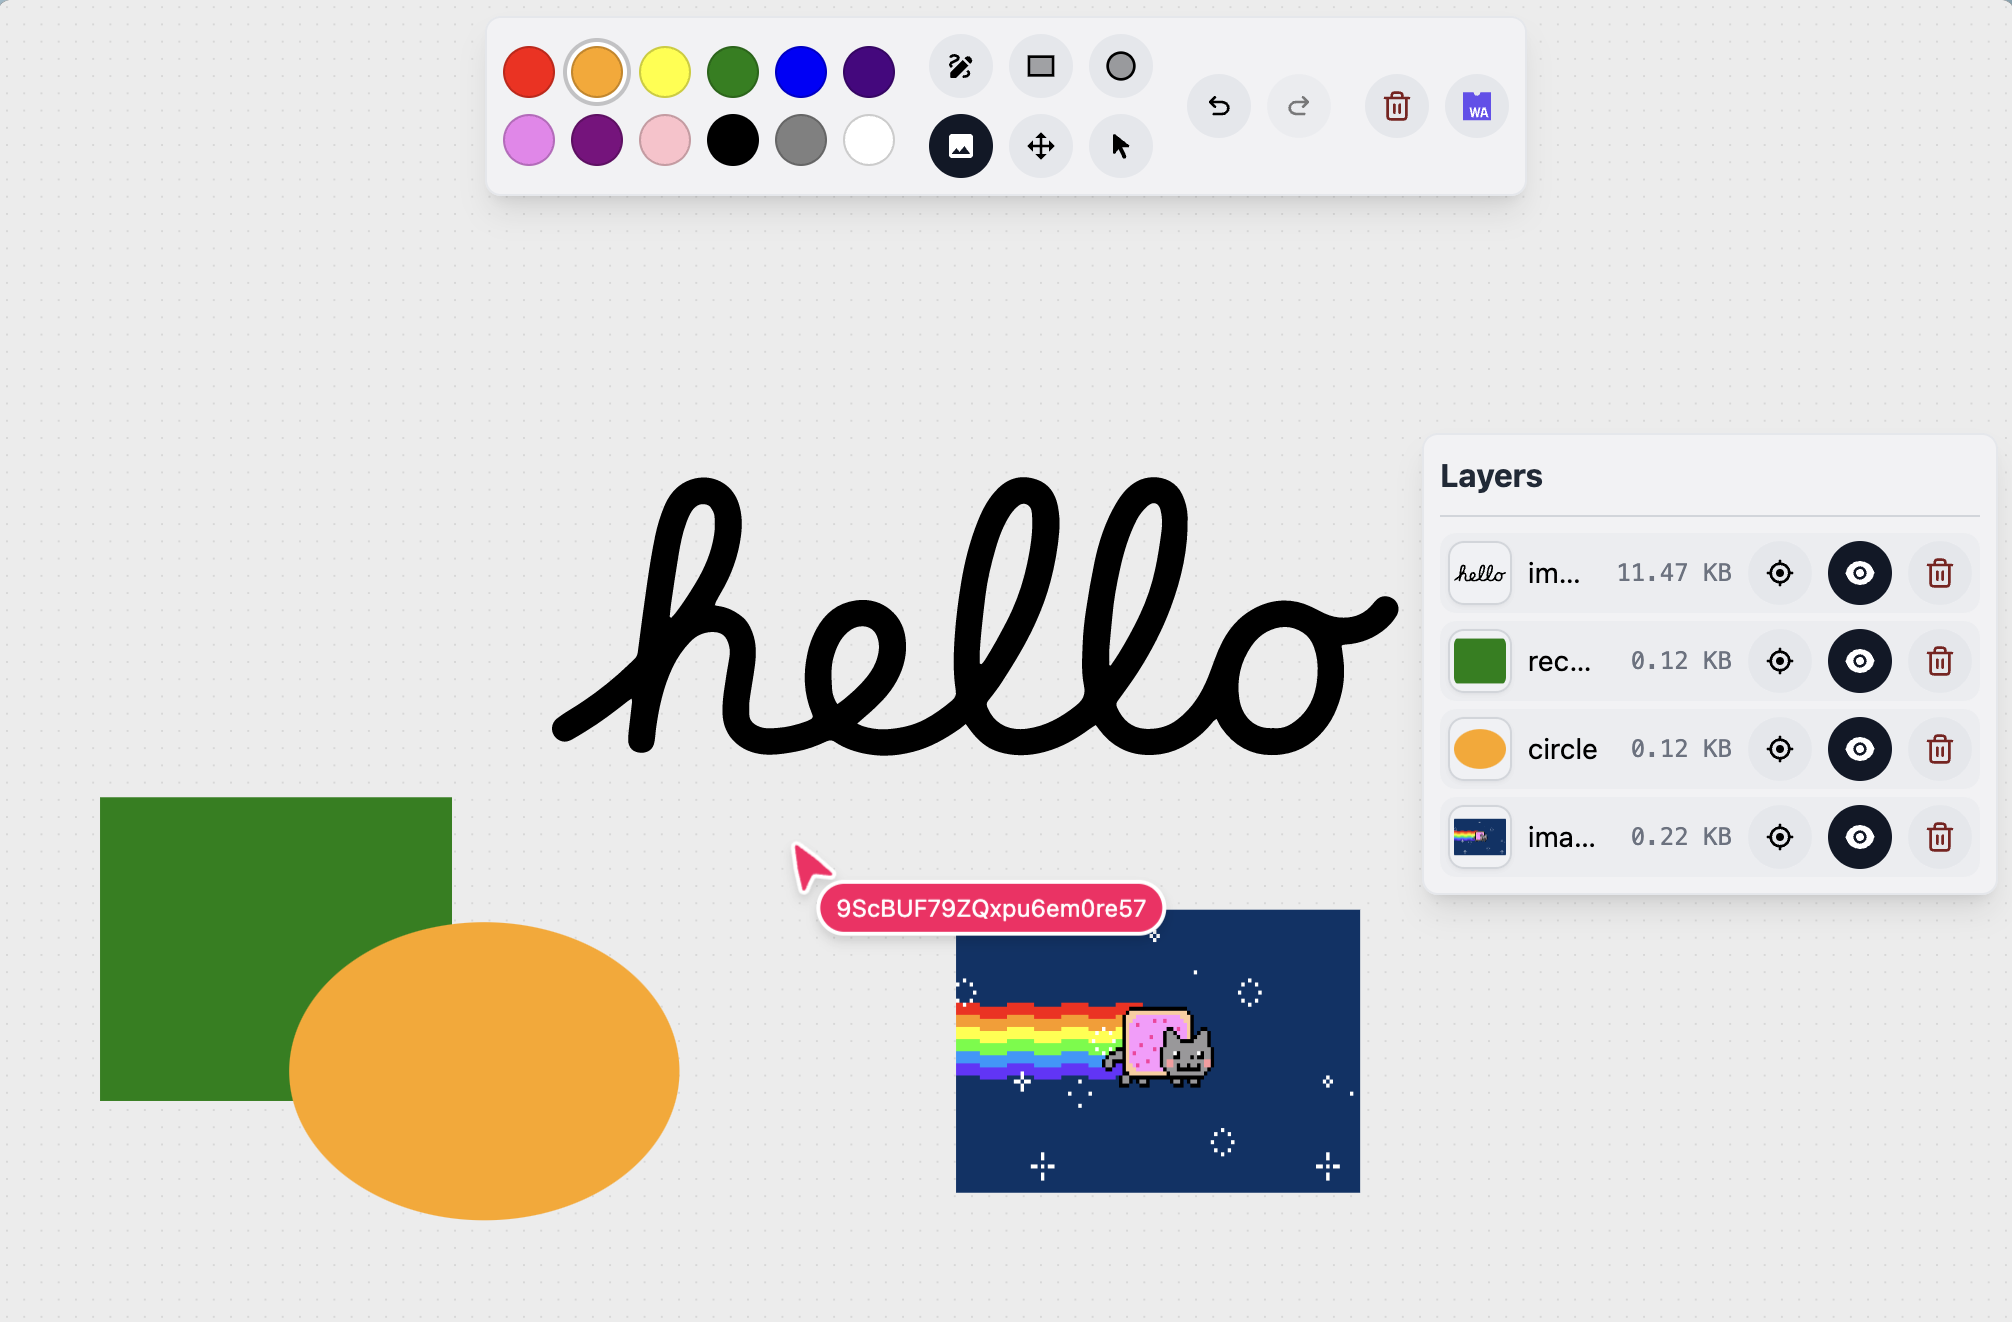
\includegraphics[width=1\textwidth]{assets/figures/whiteboard.png}
    \caption{Interface du démonstrateur Whiteboard en ligne \url{https://condensation-demo.vercel.app/}}
    \label{fig:whiteboard}
\end{figure}

Le chapitre sur le developpement du Whiteboard est encore en cours de rédaction. Il sera disponible dans la prochaine version de ce document.
Mais vous pouvez déjà consulter le code source du projet sur Github : \url{https://github.com/CondensationDS/Condensation-Monorepo} et tester le démonstrateur en ligne : \url{https://condensation-demo.vercel.app/}.

% TODO : Ajouter la conclusion
%\chapter{Conclusion}
%\section{État final du projet}

Le projet Describble s'est achevé avec succès, résultant en la création d'un tableau blanc décentralisé. Cette application offre un éventail complet de fonctionnalités de dessin, gère efficacement les documents, et est dotée d'une interface multilingue. De plus, elle a été déployée en production et répond à toutes les exigences spécifiées dans le cahier des charges révisé.

\section{Fonctionnalités additionnelles}

Au-delà des objectifs initiaux, Describble a incorporé des fonctionnalités supplémentaires qui améliorent considérablement l'expérience utilisateur. La présence en temps réel offre la possibilité de voir les curseurs des autres utilisateurs, renforçant ainsi le caractère interactif de l'application. La capacité de travailler hors ligne offre plus de flexibilité à l'utilisateur, permettant l'accès et la modification des documents même sans connexion internet. Une gestion avancée des accès aux documents a été mise en place, offrant à l'utilisateur un contrôle accru sur qui peut accéder à ses documents. En outre, l'application a été optimisée pour une utilisation sur appareils mobiles et est compatible avec les Progressive Web Applications (PWA), permettant ainsi une accessibilité et une utilisation plus larges. Enfin, l'intégration de l'internationalisation rend l'application accessible à un public plus large, transcendant les barrières linguistiques.

\section{Changements et défis rencontrés}

Initialement prévue pour une collaboration avec Condensation, cette collaboration a dû être réévaluée en raison d'une restructuration au sein de Condensation. Cela a exigé le développement d'un système de synchronisation et de réplication de données distribuées à partir de zéro, augmentant ainsi la complexité du projet. Cependant, ce défi a également permis d'acquérir des compétences techniques avancées et de bénéficier d'une expérience d'apprentissage précieuse.

\section{Apprentissages réalisés et vécu du travail de Bachelor}

Au cours de ce travail de Bachelor, j'ai acquis des compétences techniques significatives, en particulier dans le domaine de la synchronisation et de la réplication de données distribuées. La nécessité de réorienter le projet a offert une occasion d'apprendre à naviguer efficacement à travers les imprévus et à gérer les changements de direction. Malgré les défis supplémentaires engendrés par cette réorientation, ces obstacles ont été surmontés avec succès.

La réalisation de ce travail de Bachelor a été une expérience enrichissante et stimulante. L'accomplissement final, en dépit des défis rencontrés, a été d'autant plus gratifiant. Cela a non seulement renforcé mes compétences techniques, mais m'a aussi permis de gagner en résilience et en adaptabilité face aux imprévus.

\section{Remerciements}

Je tiens à exprimer ma gratitude à mon superviseur, le Professeur Bertil Chapuis. Sa guidance et son soutien tout au long de ce projet ont été précieux. Je suis également reconnaissant pour son aide dans la facilitation de la communication avec la direction de l'HEIG-VD et pour l'obtention du temps plein alloué pour ce travail de Bachelor.

J'aimerais également remercier l'équipe de Condensation. Même si notre collaboration n'a pas pu se concrétiser comme prévu, j'ai beaucoup appris grâce à eux sur le monde des startups et sur la décentralisation. Leur travail a eu une influence significative sur ce projet et m'a offert une perspective précieuse sur le potentiel de la décentralisation.

Enfin, je tiens à remercier ma famille et mes amis pour leur encouragement constant tout au long de ce parcours. Leur soutien a été une source constante d'inspiration et de motivation.

\hspace{8cm}\makeatletter\@author\makeatother\par
\hspace{8cm}\begin{minipage}{5cm}
\end{minipage}
\printsignature

\clearpage
\printbibliography

\appendix
\appendixpage
\addappheadtotoc



\let\cleardoublepage\clearpage
\backmatter

\label{glossaire}
\printnoidxglossary
\label{index}
\printindex

% Le colophon est le dernier élément d'un document qui contient des notes de l'auteur concernant la mise en page et l'édition du document : il est parfaitement optionnel.
%%%if
\clearpage
\Large\textbf{Colophon :}\par\normalsize
\thispagestyle{empty}
La qualité de cet ouvrage repose que le moteur \LaTeX. La mise en page et le format sont inspirés d'ouvrages scientifiques tels que le modèle de thèse de l'EPFL et celui des publications O'Reilly.

Les diagrammes et les illustrations sont édités depuis l'outil en ligne draw.io. Certaines illustrations ont été reprises dans Adobe Illustrator. Les représentations 3D sont exportées de SolidWorks et certains graphiques sont générés à la volée depuis un code source Python.

L'auteur fictive de ce document \emph{Maria Bernasconi} est un nom emprunté, par amusement, aux spécimens publiés par Postfinance.

Ce document a été compilé avec XeLaTeX.

La famille de police de caractères utilisée est \emph{Computed Modern} créée par Donald Knuth avec son logiciel METAFONT.
\vfil
Le Colophon est le dernier élément d'un document qui contient des notes de l'auteur concernant la mise en page et l'édition du document : il est parfaitement optionnel.
%%fi

\end{document}
